\documentclass{beamer}
\usepackage{graphicx}
\usepackage{verbatim}
\usepackage{amsmath}
\usepackage{amsfonts}
\usepackage{setspace}
% \usepackage{beamerthemesplit} // Activate for custom appearance

\title{ANOVA}
\author{Dr. Frank Wood}

\date{}

\DeclareMathOperator*{\Ave}{\mathbb{E}}
\DeclareMathOperator*{\Var}{Var}

\newcommand\independent{\protect\mathpalette{\protect\independenT}{\perp}}
\def\independenT#1#2{\mathrel{\rlap{$#1#2$}\mkern2mu{#1#2}}}
\newcommand{\argmax}{\operatornamewithlimits{argmax}}


\begin{document}

\frame{\titlepage}

\frame[t] {
 \frametitle{ANOVA}
\begin{itemize}
\item ANOVA is nothing new but is instead a way of organizing the parts of linear regression so as to make easy inference recipes.

\item Will return to ANOVA when discussing multiple regression and other types of linear statistical models.

\end{itemize}
}

\frame[t] {
 \frametitle{Partitioning Total Sum of Squares}
\begin{itemize}
\item  ``The ANOVA approach is based on the partitioning of sums of squares and degrees of freedom associated with the response variable
Y''

\item  We start with the observed deviations of $Y_i$ around the observed mean
$$Y_i - \bar{Y}$$
\end{itemize}
}

\frame[t] {
 \frametitle{Partitioning of Total Deviations}
\begin{figure}
  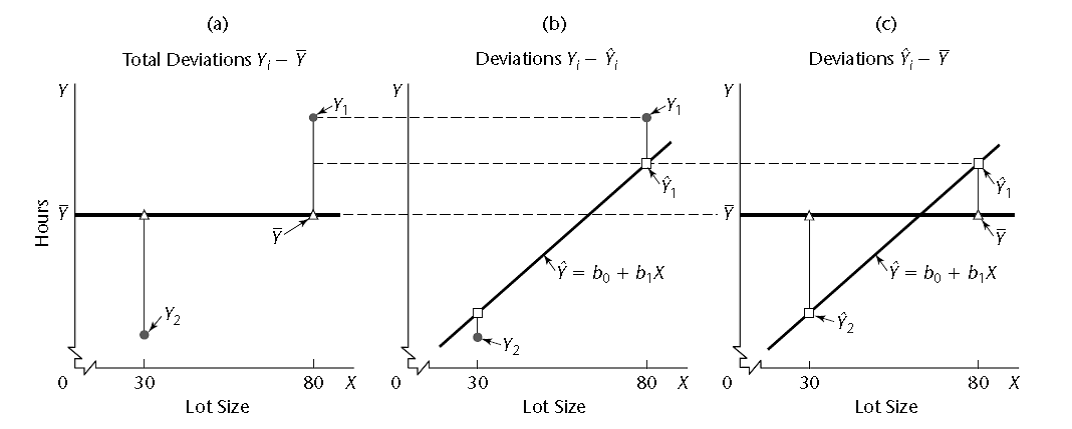
\includegraphics[height=45mm]{partition.png}
\end{figure}
}

\frame[t] {
 \frametitle{Measure of Total Variation}
\begin{itemize}
\item  The measure of total variation is denoted by $$SSTO = \sum (Y_i - \bar{Y})^2$$
\item  SSTO stands for total sum of squares
\item  If all $Y_i's$ are the same, SSTO = 0
\item  The greater the variation of the $Y_i's$ the greater SSTO
\end{itemize}
}

\frame[t] {
 \frametitle{Variation after predictor effect}
\begin{itemize}
\item  The measure of variation of the $Y_i's$ that is still present when the predictor variable X is taken into account is the sum of the squared deviations
$$SSE = \sum (Y_i - \hat{Y_i})^2$$
\item  SSE denotes error sum of squares
\end{itemize}
}

\frame[t] {
 \frametitle{Regression Sum of Squares}
\begin{itemize}
\item The difference between SSTO and SSE is SSR
$$SSR = \sum (\hat{Y_i} - \bar Y )^2$$
\item  SSR stands for regression sum of squares
\end{itemize}
}

\frame[t] { %%% DONT KNOW HOW TO CHANGE LINE IN UNDERBRACE%%%
 \frametitle{Partitioning of Sum of Squares}
\begin{eqnarray*}
\underbrace{Y_i - \bar{Y}}_{\text{Total
deviation}} =&& \underbrace{\hat{Y_i} - \bar{Y}}_{\text{Deviation of
fitted regression value around mean}}\\
 &+&
\underbrace{ Y_i -
\hat{Y_i}}_{\text{Deviation around fitted regression line}}
\end{eqnarray*} }

\frame[t] {
 \frametitle{Remarkable Property}
\begin{itemize}
\item  The sums of the same deviations squared has the same property!
$$(Y_i - \bar{Y})^2 = (\hat{Y_i} - \bar{Y})^2  + (Y_i - \hat{Y_i})^2$$or $SSTO = SSR +
SSE$
\end{itemize}
}

\frame[t] {
 \frametitle{Remarkable Property}
Proof: $(Y_i - \bar{Y})^2 = (\hat{Y_i} - \bar{Y})^2  + (Y_i -
\hat{Y_i})^2$
\begin{eqnarray*}
(Y_i - \bar{Y})^2 &=& \sum[(\hat{Y_i} - \bar{Y})  + (Y_i - \hat{Y_i})]^2 \\
&=& \sum[(\hat{Y_i} - \bar{Y})^2  + (Y_i - \hat{Y_i})^2 +2 (\hat{Y_i} - \bar{Y})(Y_i - \hat{Y_i})] \\
&=& \sum(\hat{Y_i} - \bar{Y})^2  + \sum (Y_i - \hat{Y_i})^2 +2 \sum
(\hat{Y_i} - \bar{Y})(Y_i - \hat{Y_i})
\end{eqnarray*}
but $$\sum (\hat{Y_i} - \bar{Y})(Y_i - \hat{Y_i} ) =  \sum\hat{Y_i}
(Y_i - \hat{Y_i} ) -  \sum \bar{Y} (Y_i - \hat{Y_i} ) =0$$ By
properties previously demonstrated.  Namely

$$ \sum \hat Y_i e_i = 0$$
and
$$\sum e_i = 0 $$
 }

\frame[t] {
 \frametitle{Remember: Lecture 3}
\begin{itemize}
\item  The $i^{th}$ residual is defined to be $$e_i = Y_i - \hat Y_i$$
\item  The sum of the residuals is zero:
\begin{eqnarray*}
\sum_i e_i &=& \sum(Y_i -b_0 -b_1 X_i) \\
&=& \sum Y_i - n b_0 - b_1 \sum X_i \\
&=& 0
\end{eqnarray*}
By first normal equation.
\end{itemize}
}

\frame[t] {
 \frametitle{Remember: Lecture 3}
The sum of the weighted residuals is zero when the residual in the
$i^{th}$ trial is weighted by the fitted value of the response
variable for the $i^{th}$ trial
\begin{eqnarray*}
\sum_i \hat Y_i e_i &=& \sum_i(b_0 + b_1 X_i)e_i\\
&=& b_0 \sum_i e_i + b_1 \sum_i e_i  X_i \\
&=& 0
\end{eqnarray*}
By previous properties.  The left is given by $\sum e_i = 0$, the right can be expanded to yield the second normal equation.

}

\frame[t] {
 \frametitle{Breakdown of Degrees of Freedom}
\begin{itemize}
\item SSTO
\begin{itemize}
\item 1 linear constraint due to the calculation and inclusion of the mean
\begin{itemize}
\item n-1 degrees of freedom
\end{itemize}
\end{itemize}
\item SSE
\begin{itemize}
\item 2 linear constraints arising from the estimation of $\beta_1$ and
$\beta_0$
\begin{itemize}
\item n-2 degrees of freedom
\end{itemize}
\end{itemize}
\item SSR
\begin{itemize}
\item Two degrees of freedom in the regression parameters, one is lost due to linear constraint
\begin{itemize}
\item 1 degree of freedom
\end{itemize}
\end{itemize}
\end{itemize}
}

\frame[t] {
 \frametitle{Mean Squares}
A sum of squares divided by its associated degrees of freedom is
called a mean square\\ The regression mean square is
$$MSR = \frac{SSR}{1} = SSR$$
The error mean square is
$$MSE = \frac{SSE}{n-2}$$
}

\frame[t] {
 \frametitle{ANOVA table for simple linear regression}
\begin{table}
\begin{center}
\scalebox{0.7}{
\begin{tabular}{|c|c|c|c|c|}
\hline Source of Variation& SS& df& MS & $\Ave{MS}$ \\\hline
Regression& $SSR = \sum (\hat{Y_i} - \bar Y )^2$&1&$MSR = SSR/1
$&$\sigma^2 + \beta_1^2 \sum(X_i - \bar X)^2$\\\hline Error& $SSE =
\sum (Y_i - \hat{Y_i})^2$&$n-2$&$MSE = SSE/(n-2)
$&$\sigma^2$\\\hline Total& $SSTO = \sum (Y_i -
\bar{Y})^2$&$n-1$&&\\\hline
\end{tabular}}
\end{center}
\end{table}
}

\frame[t] {
 \frametitle{$\Ave{MSE} = \sigma^2$}
\begin{itemize}
\item Remember the following theorem, presented in an earlier lecture.
\bigskip

For the normal error regression model, $\frac{SSE}{\sigma^2}$ is distributed as $\chi^2$ with $n-2$ degrees of freedom and is independent of both $b_0$ and $b_1$.
\bigskip

 Rewritten this yields $$SSE/\sigma^2 \sim \chi^2(n-2)
$$
\item That means that $\Ave{SSE/\sigma^2} = n-2$
\item And thus that $\Ave{SSE/(n-2)} = \Ave{MSE} = \sigma^2$
\end{itemize}
}

\frame[t] {
 \frametitle{$E\{MSR\} = \sigma^2 + \beta_1^2 \sum(X_i - \bar X)^2$}
\begin{itemize}
\item To begin, we take an alternative but equivalent form for SSR
$$SSR = b_1^2 \sum(X_i - \bar X)^2$$
\item And note that, by definition of variance we can write
$$\sigma^2\{b_1\} = E\{b_1^2\} - (E\{b_1\})^2$$
\end{itemize}
}

\frame[t] {
 \frametitle{$E\{MSR\} = \sigma^2 + \beta_1^2 \sum(X_i - \bar X)^2$}
\begin{itemize}
\item But we know that $b_1$ is an unbiased estimator of $\beta_1$ so $\Ave{b_1} =
\beta_1$
\item We also know (from previous lectures) that
$$\sigma^2\{b_1\} = \frac{\sigma^2}{\sum(X_i - \bar X)^2}$$
\item So we can rearrange terms and plug in
\begin{eqnarray*}
\sigma^2\{b_1\} &=& E\{b_1^2\} - (E\{b_1\})^2 \\
E\{b_1^2\} &=& \frac{\sigma^2}{\sum(X_i - \bar X)^2} +\beta_1^2
\end{eqnarray*}
\end{itemize}
}

\frame[t] {
 \frametitle{$E\{MSR\} = \sigma^2 + \beta_1^2 \sum(X_i - \bar X)^2$}
\begin{itemize}
\item From the previous slide\begin{eqnarray*}
E\{b_1^2\} &=& \frac{\sigma^2}{\sum(X_i - \bar X)^2} +\beta_1^2
\end{eqnarray*}
\item  Which brings us to our desired result\\
\end{itemize}
\[E\{MSR\} = E\{SSR/1\} = E\{b_1^2\}\sum(X_i - \bar X)^2  =
 \sigma^2 + \beta_1^2 \sum(X_i - \bar X)^2\]
}

\frame[t] {
 \frametitle{Comments and Intuition}
\begin{itemize}
\item The mean of the sampling distribution of MSE is
$\sigma^2$ regardless of whether X and Y are linearly related (i.e.
whether $\beta_1 = 0$)

\item The mean of the sampling distribution of MSR is also $\sigma^2$ when $\beta_1 = 0$.
\begin{itemize}
\item When $\beta_1 = 0$ the sampling distributions of MSR and MSE tend to be the same

\end{itemize}
\end{itemize}
This intuition leads us to a battery of simple rules for constructing linear regression tests
}

\frame[t] {
 \frametitle{F Test of $\beta_1 = 0$ vs. $\beta_1 \neq 0$}
ANOVA provides a battery of useful tests.  For example, ANOVA
provides an easy test for
\bigskip
\begin{columns}
\begin{column}{.5\linewidth}
Two-sided test
\begin{eqnarray*}
H_0 &:&  \beta_1 = 0\\
H_a &:&  \beta_1 \neq 0
\end{eqnarray*}
\end{column}
\begin{column}{.5\linewidth}
Two-sided t-test statistic from before\\
\[t^* = \frac{b_1-0}{s\{b_1\}}\]
ANOVA test statistic
\[F^* = \frac{MSR}{MSE}\]
\end{column}
\end{columns}
\vspace{10mm}

The ANOVA framework makes many common linear regression tests into almost ``shorthand.''
}

\frame[t] {
 \frametitle{Sampling distribution of $F^*$}
\begin{itemize}
\item The sampling distribution of $F^*$ when $H_0 : \beta_1 = 0$ holds can be derived starting from Cochran's theorem
\end{itemize}
\begin{block}{Cochran's theorem}
If all n observations $Y_i$ come from the same normal distribution
with mean $\mu$ and variance $\sigma^2$, and SSTO is decomposed into
k sums of squares $SS_r$, each with degrees of freedom $df_r$, then
the $SS_r/\sigma^2$ terms are independent $\chi^2$ variables with
$df_r$ degrees of freedom if
$$\sum_{r=1}^k df_r = n-1$$
\end{block}
Does this directly apply to the regression case?


}

\frame[t] {
 \frametitle{The F Test}
We have decomposed SSTO into two sums of squares SSR and SSE and
their degrees of freedom are additive, hence, by Cochran's theorem:
If $\beta_1 = 0$ so that all $Y_i$ have the same mean $\mu=\beta_0$
and the same variance $\sigma^2$, $SSE/\sigma^2$ and $SSR/\sigma^2$
are independent $\chi^2$ variables }

\frame[t] {
 \frametitle{$F^*$ Test Statistic}
\begin{itemize}
\item $F^*$ can be written as follows$$F^* =  \frac{MSR}{MSE} = \frac{\frac{SSR/\sigma^2}{1}}{  \frac{SSE/\sigma^2}{n-2} }$$
\item But by Cochran' s theorem, we have when $H_0$ holds$$F^* \sim \frac{\frac{\chi^2(1)}{1}}{\frac{\chi^2(n-2)}{n-2}}$$
\end{itemize}
}

\frame[t] {
 \frametitle{F Distribution}
\begin{itemize}
\item The F distribution is the ratio of two independent $\chi^2$ random variables.

\item The test statistic $F^*$ follows the distribution\\$F^* \sim F(1,n-2)
$
\end{itemize}
}

\frame[t] {
 \frametitle{Hypothesis Test Decision Rule}
Since $F^*$ is distributed as $F(1,n-2)$ when $H_0$ holds, the
decision rule to follow when the risk of a Type I error is to be
controlled at $\alpha$ is:\\
\bigskip
If $F^* \leq F(1-\alpha; 1, n-2)$, conclude $H_0$\\
If $F^* > F(1-\alpha; 1, n-2)$, conclude $H_a$ }

\frame[t] { %%%change pic%%%
 \frametitle{F distribution}
\begin{itemize}
\item PDF, CDF, Inverse CDF of F distribution
\begin{figure}
  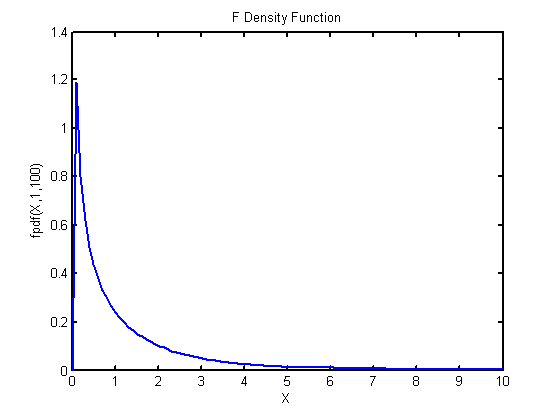
\includegraphics[height=20mm]{f1.png}
  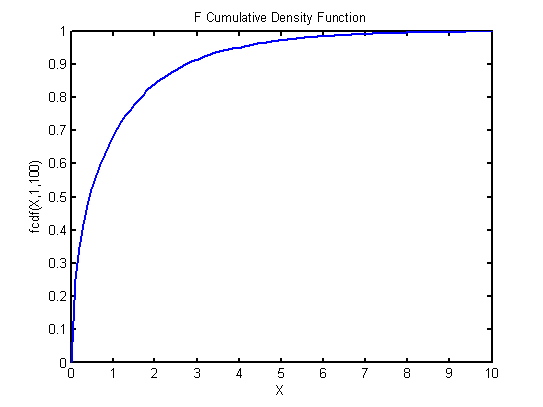
\includegraphics[height=20mm]{f2.png}
  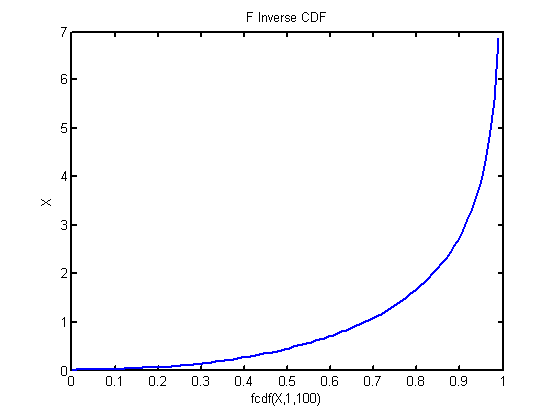
\includegraphics[height=20mm]{f3.png}
\end{figure}
\item Note, MSR/MSE must be big in order to reject hypothesis.

\end{itemize}
}

\frame[t] {
 \frametitle{Partitioning of Total Deviations}
Does this make sense?  When is MSR/MSE big?
\begin{figure}
  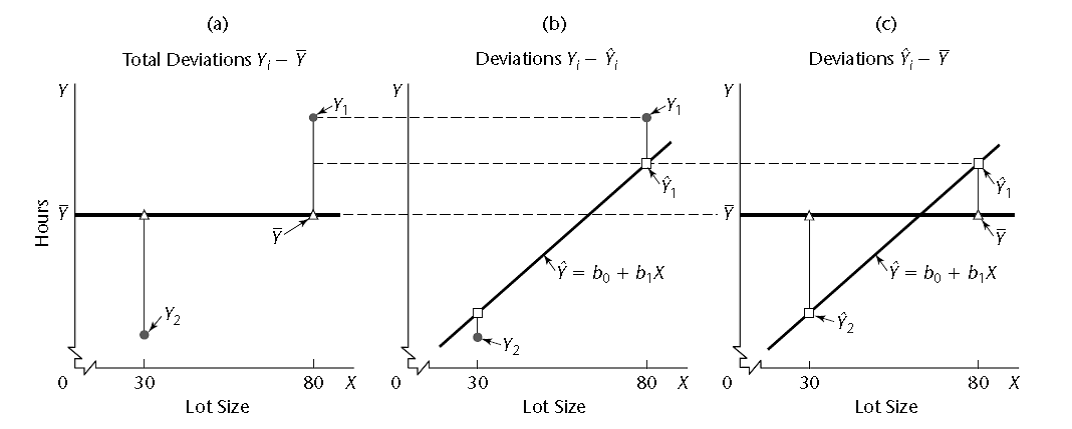
\includegraphics[height=40mm]{msr.png}
\end{figure} }

\frame[t] {
 \frametitle{General Linear Test}
\begin{itemize}
\item The test of $\beta_1=0$ versus $\beta_1\neq 0$ is but a single example of
a general test for a linear statistical models.
\item The general linear test has three parts
\begin{itemize}
\item Full Model
\item Reduced Model
\item Test Statistic
\end{itemize}
\end{itemize}
}

\frame[t] {
 \frametitle{Full Model Fit}
\begin{itemize}
\item A full linear model is first fit to the
data$$Y_i = \beta_0 + \beta_1 X_i + \epsilon_i$$
\item Using this model the error sum of squares is obtained, here for example the simple linear model with non-zero slope is the ``full'' model
$$SSE(F) = \sum[Y_i - (b_0 + b_1 X_i)]^2 = \sum (Y_i - \hat Y_i)^2 = SSE$$
\end{itemize}
}

\frame[t] {
 \frametitle{Fit Reduced Model}
\begin{itemize}
\item One can test the hypothesis that a simpler model is a ``better'' model via a general linear test (which is really a likelihood ratio test in disguise).  For instance, consider a ``reduced'' model in which the slope is zero (i.e. no relationship between input and output).   \\
\bigskip
$H_0: \beta_1=0$\\
$H_a: \beta_1\neq 0$
\bigskip
\item The model when $H_0$ holds is called the reduced or restricted model.
$$Y_i = \beta_0 + \epsilon_i$$
\item The SSE for the reduced model is obtained$$SSE(R) = \sum(Y_i-b_0)^2 = \sum(Y_i - \bar Y)^2 = SSTO$$
\end{itemize}
}

\frame[t] {
 \frametitle{Test Statistic}
\begin{itemize}
\item The idea is to compare the two error sums of squares SSE(F) and SSE(R).
\item Because the full model F has more parameters than the reduced model R $SSE(F) \leq SSE(R)$ always

\item In the general linear test, the test statistic is
$$F^* = \frac{\frac{SSE(R)-SSE(F)}{df_R - df_F}}{\frac{SSE(F)}{df_F}}$$which follows the F distribution when $H_0$ holds.
\item $df_R$ and $df_F$ are those associated with the reduced and full model error sums of square respectively
\end{itemize}
}

\frame[t] {
 \frametitle{$R^2$}
\begin{itemize}
\item SSTO measures the variation in the observations $Y_i$ when X is not considered
\item SSE measures the variation in the $Y_i$ after a predictor variable X is employed
\item A natural measure of the effect of X in reducing variation in Y is to express
the reduction in variation $(SSTO-SSE = SSR)$ as a proportion of the
total variation$$R^2 = \frac{SSR}{SSTO} = 1 - \frac{SSE}{SSTO}$$
\item Note that since $ 0 \leq SSE \leq SSTO$ then $0\leq R^2\leq 1$
\end{itemize}
}

\frame[t] {
 \frametitle{Limitations of and misunderstandings about $R^2$}
\begin{enumerate}
\item Claim: high $R^2$ indicates that useful predictions can be made.  The prediction interval for a particular input of interest may still be wide even if $R^2$ is high.
\item Claim: high $R^2$ means that there is a good linear fit between predictor and output.  It can be the case that an approximate (bad) linear fit to a truly curvilinear relationship might result in a high $R^2$.
\item Claim: low $R^2$ means that there is no relationship between input and output.  Also not true since there can be clear and strong relationships between input and output that are not well explained by a linear functional relationship.
\end{enumerate}
}

\end{document}
